\documentclass[a4paper]{article}

%% Language and font encodings
\usepackage[french]{babel}
\usepackage[utf8x]{inputenc}
\usepackage[T1]{fontenc}

%% Sets page size and margins
\usepackage[a4paper,top=3cm,bottom=3cm,left=2cm,right=2cm,marginparwidth=2cm]{geometry}

%% Useful packages
\usepackage{amsmath}
\usepackage{graphicx}
\usepackage[colorinlistoftodos]{todonotes}
\PassOptionsToPackage{hyphens}{url}
\usepackage[colorlinks=true, allcolors=black]{hyperref}
\usepackage{fourier-orns}
\usepackage{titlesec}
\usepackage{fancyhdr}
\usepackage{fancyvrb}
\pagestyle{fancy} 
\setcounter{tocdepth}{5}
\usepackage{fancyvrb}

%% Pour les exemples
\usepackage{mdframed}
\newmdenv[topline=false, bottomline=false, rightline=false, skipabove=\topsep, skipbelow=\topsep]{example}

%% Tikz stuff
\usepackage{tikz}
\usetikzlibrary{calc, arrows}
\tikzstyle{incolore} = [rectangle, rounded corners, draw=black, minimum height=1cm, minimum width=3cm, text width=3cm, text centered]

\usepackage{libertine}
\newcommand{\hsp}{\hspace{20pt}}
\newcommand{\HRule}{\rule{\linewidth}{0.5mm}}

\renewcommand{\headrulewidth}{1pt}
\fancyhead[C]{} 
\fancyhead[L]{}
\fancyhead[R]{\footnotesize{\leftmark}}

\renewcommand{\footrulewidth}{1pt}
\fancyfoot[C]{} 
\fancyhead[L]{}
\fancyfoot[R]{\thepage}

\definecolor{Zgris}{rgb}{0.87,0.85,0.85}

\usepackage{eso-pic,graphicx}
\usepackage{xcolor}
\newcommand{\bgimg}[1]
{
    \AddToShipoutPicture
    {
        \put(\LenToUnit{0 cm},\LenToUnit{0 cm})
        {
            \includegraphics[width=\paperwidth,height=\paperheight]{#1}
        }
    }
}

%% To list and caption code
\usepackage{minted}
\renewcommand{\listoflistingscaption}{Table des programmes}
\usepackage{caption}
\newenvironment{code}{\captionsetup{type=listing}}{}
\renewcommand{\listingscaption}{Programme}

\begin{document}




\begin{titlepage}
    \begin{sffamily}
        \begin{center}

            
\includegraphics[width=5cm]{images/LogoHenallux.png}~\\[1.5cm]
            \textsc{\Large Rapport travail en autonomie}\\[1.5cm]

            \HRule \\[0.4cm]
            { \huge \bfseries Système de fichier : NTFS\\[0.4cm] }
            \HRule \\[2cm]

            \begin{minipage}{0.4\textwidth}
                \begin{flushleft} \large
                    Roumache Grégoire\\
                    Sénéchal Julien\\
                    Wallemme Maxime\\
                \end{flushleft}
            \end{minipage}
            \begin{minipage}{0.55\textwidth}
                \begin{flushright} \large
                    IR317 - Forensics and cyberattack evidence 2021-2022\\
                    Sécurité des systèmes, Hénallux\\
                    Troisième année, Classe A Groupe 1 \\
                \end{flushright}
            \end{minipage}
            \vfill

            {\large 09 Novembre 2021}

        \end{center}
    \end{sffamily}
\end{titlepage}

\let\cleardoublepage\clearpage










\section{Introduction}

Le système de fichiers NTFS (New Technology File System) est le système de fichier de Microsoft, il succède au système de fichier FAT. Il est plus performant en termes de vitesse et d'utilisation du disque. Il est aussi plus fiable grâce à l'utilisation d'un système de journalisation. Son support des métadonnées est aussi très intéressant et nous allons nous y intéresser dans ce rapport.










\section{Principes de fonctionnement}



\subsection{Fichiers système}

Avec NTFS tout est un fichier, y compris les données utilisées par le système de fichier lui-même. On les appelle les fichiers systèmes, ils se situent à la racine et sont cachés parce que leurs noms commencent par un dollar \$.

Il y a deux types d'index dans NTFS, la MFT (\textbf{M}aster \textbf{F}ile \textbf{T}able) qui contient la liste de tous les fichiers sur le système, dont elle-même. Il y a aussi les index I30 qui se trouvent dans chaque dossier et contiennent la liste des fichiers du dossier dans lequel ils se trouvent. 



\subsection{Métadonnées}

La MFT contient les métadonnées du système. Voici les attributs qu'un fichier peut avoir :
\begin{center}
    \begin{tabular}{|l|l|} \hline
        \textbf{Attribut}           & \textbf{Description} \\ \hline
        Nom                & Nom du fichier \\
        Taille             & Taille du fichier sur le disque \\
        Horodatage         & Date et heure de dernier accès, dernière modification et création \\
        ACL                & Liste de permissions pour contrôler l'accès au fichier \\
        Adresse du fichier & Précise l'endroit sur le disque qui contient les données du fichier \\ \hline
    \end{tabular}
\end{center}

NTFS note quelle opération va être lancée avant de l'exécuter. Par exemple, il va écrire dans les logs qu'il va supprimer un fichier avant de le supprimer. Ça permet d'achever correctement la transaction si la machine redémarre en plein pendant la suppression.



\subsection{Flux alternatifs}

Les fichiers NTFS peuvent avoir plusieurs flux (*streams* en anglais). Chaque fichier a un flux de données {\small \texttt{:\$DATA}} qui contient les données du fichier. Cependant, il peut aussi avoir d'autres flux, appelé flux de données alternatif contenant des données pas directement visible à l'utilisateur. Exemple avec des commandes CMD:
\begin{example}
\begin{Verbatim}[fontsize=\small]
echo test > test.txt
echo hello > test.txt:hello
dir
more < test.txt
more < test.txt:hello
del test.txt
dir
\end{Verbatim}
\end{example}
Ici, nous a créé le fichier \textit{test.txt} et on a mis:
\begin{itemize}
    \item "test" dans le flux {\small \texttt{:\$DATA}}
    \item "hello" dans le flux {\small \texttt{hello}}
\end{itemize}
Ensuite, nous avons bien vérifié qu'il n'y avait qu'un seul fichier présent. Nous avons lu les données des deux flux. Et nous avons supprimé le fichier. Une fois supprimé, aucun des deux flux n'est plus accessible.









\newpage
\section{Outils d'analyses}


\subsection{FTK Imager}

Cet outil permet d'analyser l'entièreté d'un système de fichiers NTFS. Celui-ci peut vous permettre de retrouver, par exemple, le \emph{\$MFT} qui contient tous les enregistrements des fichiers stockés et leurs informations (nom, horodatage, type de fichier, etc.) comme on peut le voir à la figure \ref{fig:ftk}. Il s'agit d'un élément crucial de l’investigation numérique, car elle permet de retracer les évènements.

\begin{figure}[H]
    \centering
    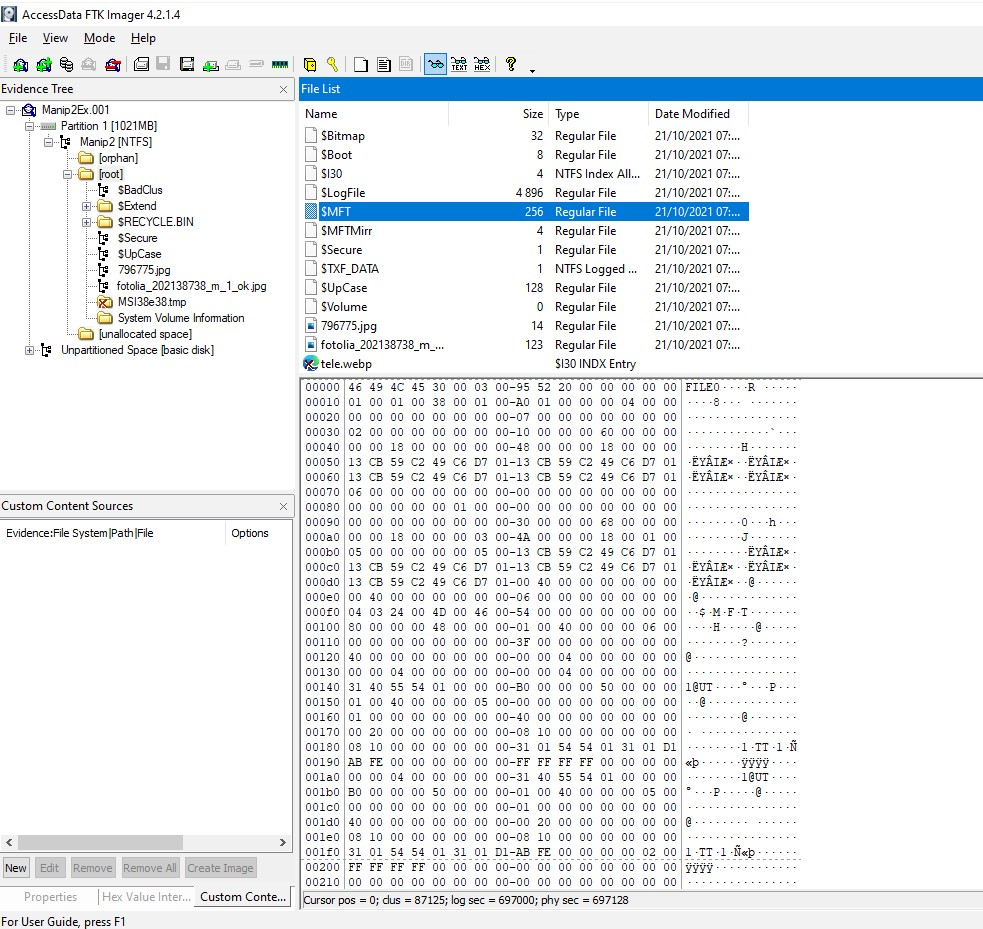
\includegraphics[width=0.99\linewidth]{images/ftk.jpg}
    \caption{Découverte du \$MFT avec FTK Imager}
    \label{fig:ftk}
\end{figure}

\subsection{Mft2Csv}
Il s'agit d'un outil permettant de décoder les données et de traiter les données contenues dans le \$MFT (Voir Figure \ref{mft1}). Une fois le traitement terminé, nous obtenons un fichier en format CSV. Le CSV va nous permettre la facilité de lecture (une fois la mise en page adaptée) et ainsi pouvoir inspecter la chronologie des évènements (Voir Figure \ref{mft2}).

\begin{figure}[H]
    \centering
    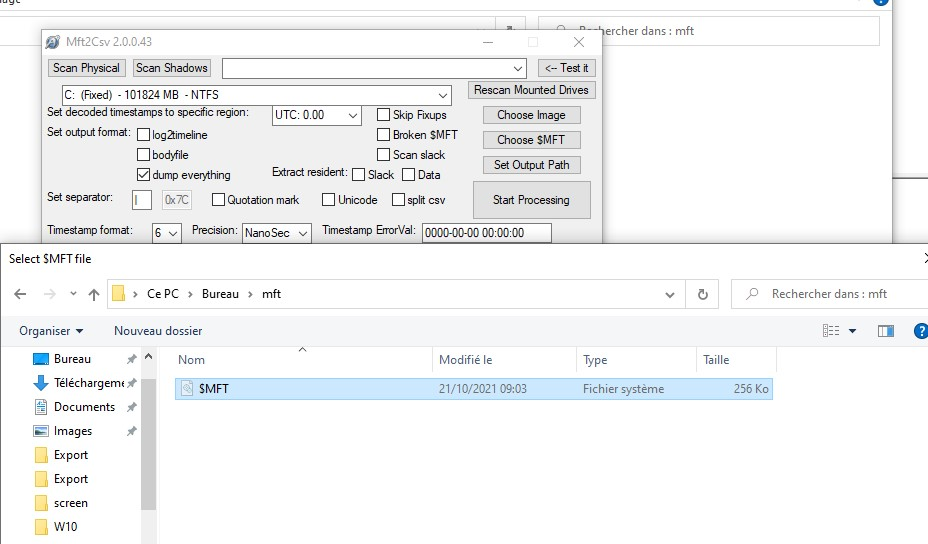
\includegraphics[width=0.59\linewidth]{images/mft1.jpg}
    \caption{Analyse de la Master File Table}
    \label{mft1}
\end{figure}

\begin{figure}[H]
    \centering
    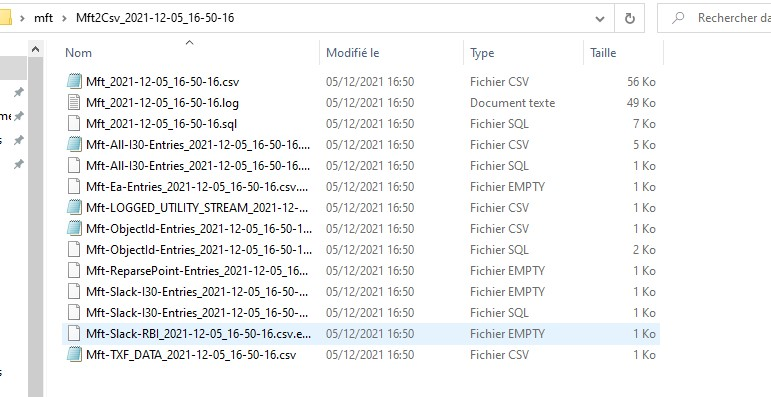
\includegraphics[width=0.99\linewidth]{images/mft2.jpg}
    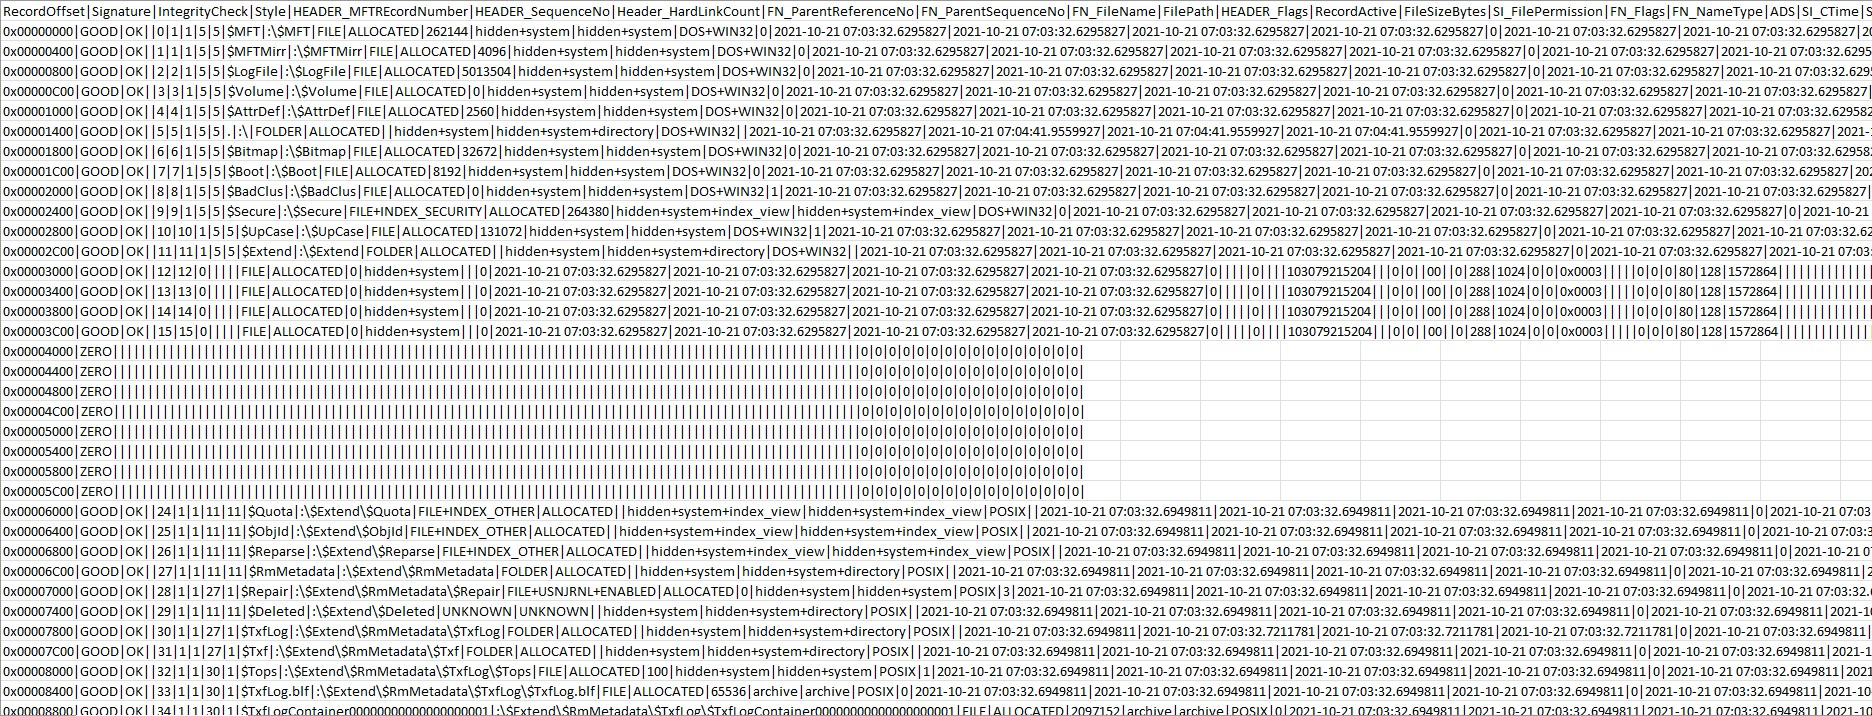
\includegraphics[width=0.99\linewidth]{images/mft3.jpg}
    \caption{Exportation en CSV de la MFT}
    \label{mft2}
\end{figure}


\subsection{Autopsy}

Avec Autopsy, on peut également analyser les fichiers du système de fichiers NTFS. Pour illustrer cette analyse, nous avons surligner, sur la figure \ref{fig:autopsy}, une image supprimée. On peut voir le flux principal \textit{\$RORROW3.jfif}, le flux alternatif \textit{Zone.Identifier} et \textit{\$IORROW3.jfif} qui contient le chemin du fichier comme vous pouvez le voir à la figure \ref{fig:autopsy2}.

\begin{figure}[H]
    \centering
    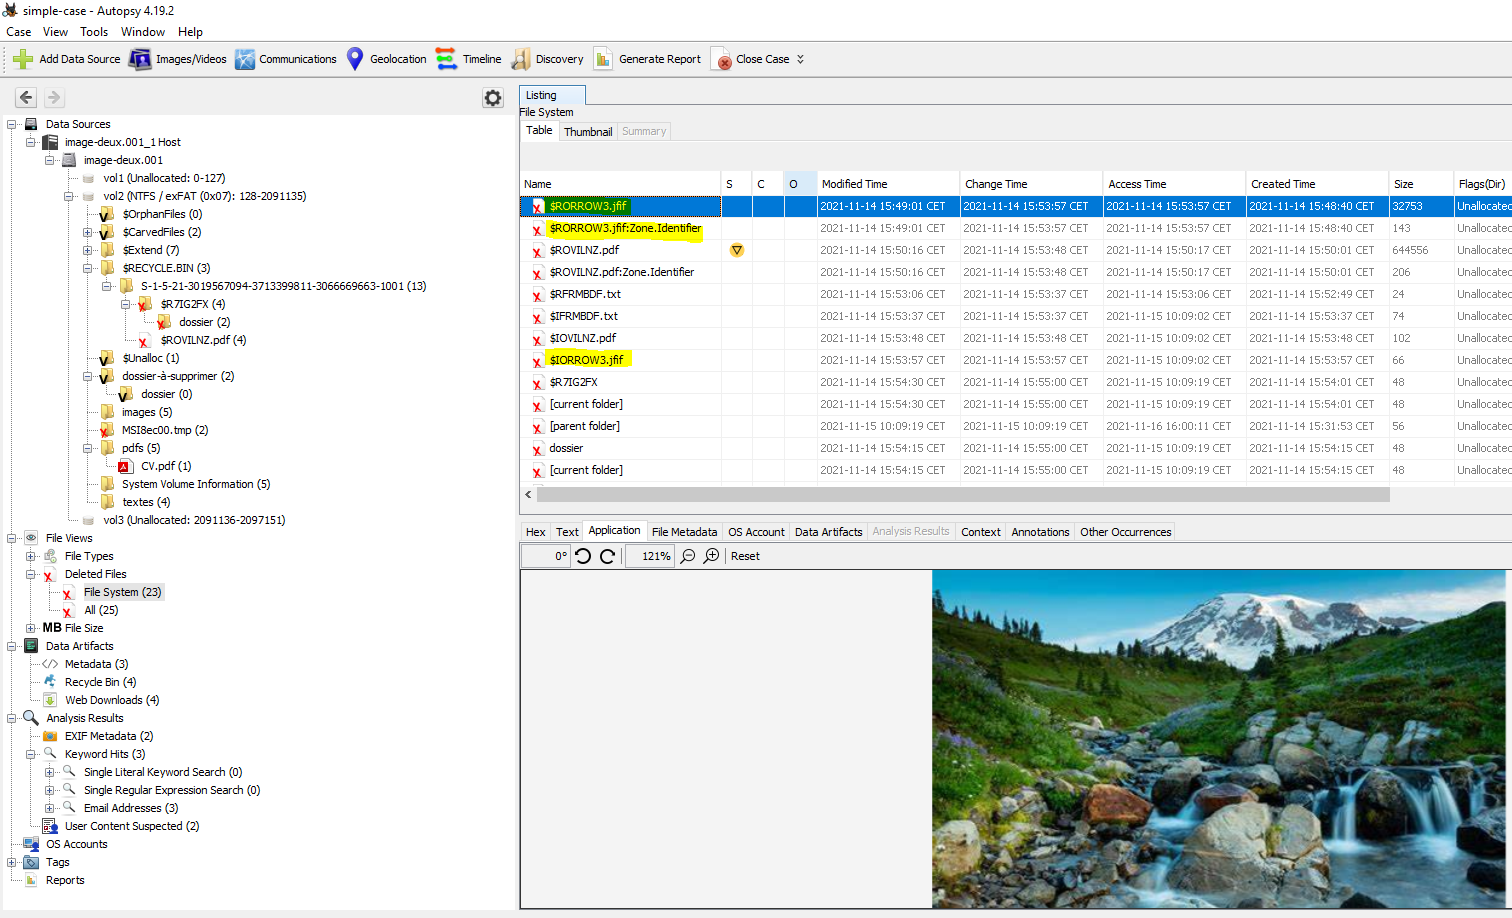
\includegraphics[width=0.99\linewidth]{images/004-autopsy.PNG}
    \caption{Analyse d'un fichier supprimé avec Autopsy}
    \label{fig:autopsy}
\end{figure}

\begin{figure}[H]
    \centering
    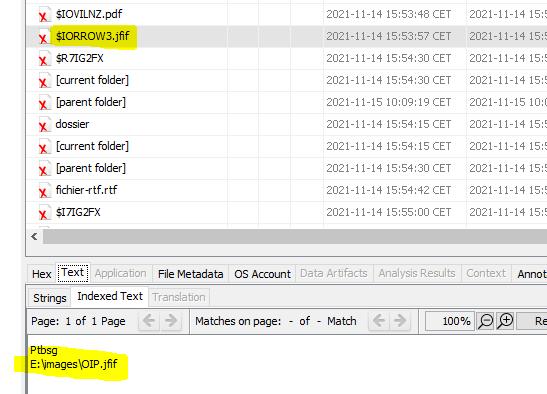
\includegraphics[width=10cm]{images/007-autopsy.PNG}
    \caption{Métadonnées contenant le chemin du fichier supprimé}
    \label{fig:autopsy2}
\end{figure}









\section{Exemple de métadonnées que l'on peut trouver pour un fichier}
Sur le système de fichier NTFS, on peut retrouver différentes métadonnées pour un fichier comme:
\begin{itemize}
    \item Nom
    \item Type de fichier
    \item Le chemin du dossier dans lequel il se situe
    \item La taille du fichier
    \item La date de création et de modification
    \item Les attributs du fichier : Ceux-ci permettent de donner une fonction à un fichier (exemple: l'attribut H permet de caché le fichier même lorsque la commande dir est utilisée.).\\
    Dans mon cas, l'attribut A permet de marquer le fichier comme créé ou modifié après la dernière sauvegarde.
    \item Le propriétaire du fichier
    \item L'ordinateur sur lequel le fichier à été créé
\end{itemize}

\begin{figure}[H]
    \centering
    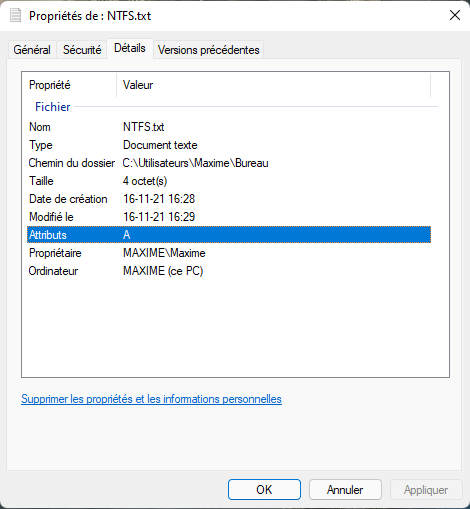
\includegraphics[width=8cm]{images/metadata_ntfs.png}
    \caption{Exemples de métadonnées d'un fichier sur NTFS}
    \label{fig:metadata_ntfs}
\end{figure}








\section{Conclusion}
Nous avons eu l'occasion de faire un rapide tour du système de conclusion. En effet, nous avons tout d'abord pu voir le principe de fonctionnement de NTFS tel que l'utilité de sa master file table, de ses métadonnées ou encore en découvrant les flux alternatifs. Ensuite, nous avons pu découvrir 3 outils intéressant dans le processus d'analyse de ce système de fichiers. Et enfin, nous avons pu avoir un avant-goût d'une analyse du système de fichiers en utilisant Autopsy.




















\end{document}